\begin{pa} \label{PA:10.8}  According to U.S.~postal regulations, the girth plus the length of a parcel sent by mail may not exceed 108 inches, where by ``girth'' we mean the perimeter of the smallest end.  Our goal is to find the largest possible volume of a rectangular parcel with a square end that can be sent by mail.\footnote{We solved this applied optimization problem in single variable \emph{Active Calculus}, so it may look familiar. We take a different approach in this section, and this approach allows us to view most applied optimization problems from single variable calculus as constrained optimization problems, as well as provide us tools to solve a greater variety of optimization problems.} If we let $x$ be the length of the side of one square end of the package and $y$ the length of the package, then we want to maximize the volume $f(x,y) = x^2y$ of the box subject to the constraint that the girth ($4x$) plus the length ($y$) is as large as possible, or $4x+y = 108$.  The equation $4x + y = 108$ is thus an external constraint on the variables. 
    \ba
    \item The constraint equation involves the function $g$ that is given by
    \[g(x,y) = 4x+y.\]
    Explain why the constraint is a contour of $g$, and is therefore a two-dimensional curve.

  \begin{figure}[ht]
  \begin{center}
    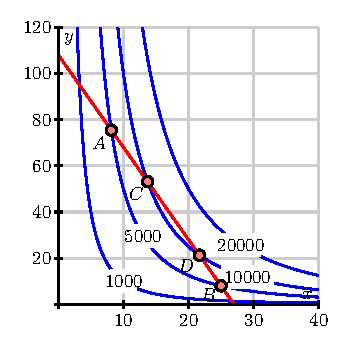
\includegraphics{figures/fig_10_8_postal.eps}
  \end{center}
  \caption{Contours of $f$ and the constraint equation $g(x,y) = 108$.}
  \label{F:10.8.preview}
  \end{figure}

    \item Figure \ref{F:10.8.preview} shows the graph of the constraint equation $g(x,y) = 108$ along with a few contours of the volume function $f$.  Since our goal is to find the maximum value of $f$ subject to the constraint $g(x,y) = 108$, we want to find the point on our constraint curve that intersects the contours of $f$ at which $f$ has its largest value. 
	\begin{enumerate}[i.]
	\item Points $A$ and $B$ in Figure \ref{F:10.8.preview} lie on a contour of $f$ and on the constraint equation $g(x,y) = 108$. Explain why neither $A$ nor $B$ provides a maximum value of $f$ that satisfies the constraint. 
	\item Points $C$ and $D$ in Figure \ref{F:10.8.preview} lie on a contour of $f$ and on the constraint equation $g(x,y) = 108$. Explain why neither $C$ nor $D$ provides a maximum value of $f$ that satisfies the constraint. 
	\item Based on your responses to parts i. and ii., draw the contour of $f$ on which you believe $f$ will achieve a maximum value subject to the constraint $g(x,y) = 108$. Explain why you drew the contour you did. 
	\end{enumerate}
	

\item Recall that $g(x,y) = 108$ is a contour of the function $g$, and that the gradient of a function is always orthogonal to its contours. With this in mind, how should $\nabla f$ and $\nabla g$ be related at the optimal point? Explain. 


    \ea
\end{pa} 

\begin{activitySolution} 
    \ba
    \item A contour is a curve obtained by setting the dependent variable equal to a constant. So if $g(x,y) = 4x+y$, then the equation $108 = 4x+y = g(x,y)$ is a contour of $g$.


    \item Notice that there are contours of $f$ that intersect the constraint with higher values of $f$ than occur at points $A$, $B$, $C$, or $D$. It appears that that maximum value of $f$ that we want will occur at a point where the contour of $f$ intersects the constraint at only one point -- or when the contour of $f$ is tangent to the constraint.


\item When the graph of the constraint is tangent to a level curve of $f$, then the two curves will have the same direction at this point. This implies any two vectors that are orthogonal to these level curves will have to be parallel at the point of tangency. So $\nabla f$ and $\nabla g$ will have to be parallel at the point of tangency.


    \ea
\end{activitySolution}
\afterpa 